% Modelo de TCC do Bacharelado em Ciência da Computação da UNIFESP 
% Baseado no Modelo de Documentos Academicos do ABNTex2  

\documentclass[	12pt, Times, openright, twoside, a4paper, english, brazil]{abntex2}

% ---
% Pacotes fundamentais 
% ---
\usepackage{cmap}				% Mapear caracteres especiais no PDF
%\usepackage{lmodern}			% Usa a fonte Latin Modern			
\usepackage{times}
\usepackage[T1]{fontenc}			% Selecao de codigos de fonte.
\usepackage[utf8]{inputenc}		% Codificacao do documento (conversão automática dos acentos)
\usepackage{lastpage}			% Usado pela Ficha catalográfica
%\usepackage{natbib}
\usepackage{indentfirst}			% Indenta o primeiro parágrafo de cada seção.
\usepackage{color}				% Controle das cores
\usepackage{graphicx}			% Inclusão de gráficos
% ---

% ---
% Pacotes de citações
% ---
\usepackage[brazilian,hyperpageref]{backref}	 % Paginas com as citações na bibl
\usepackage[alf]{abntex2cite}	% Citações padrão ABNT

% --- 
% CONFIGURAÇÕES DE PACOTES
% --- 

% ---
% Configurações do pacote backref
% Usado sem a opção hyperpageref de backref
\renewcommand{\backrefpagesname}{Citado na(s) página(s):~}
% Texto padrão antes do número das páginas
\renewcommand{\backref}{}
% Define os textos da citação
\renewcommand*{\backrefalt}[4]{
	\ifcase #1 %
		Nenhuma citação no texto.%
	\or
		Citado na página #2.%
	\else
		Citado #1 vezes nas páginas #2.%
	\fi}%
% ---

% numeração de figuras e tabelas 
\counterwithout{figure}{section}
\counterwithout{table}{section}

%\renewcommand\tablename{Tabela{\arabic{chapter}.}}


% ---
% Informações de dados para CAPA e FOLHA DE ROSTO
% ---
\titulo{Predição de propriedades para materiais 2D usando aprendizado contrastivo}
% \titulo{Property Prediction for 2D Materials using Contrastive Learning}
\autor{Luis Filipe Carvalho de Menezes}
\local{São José dos Campos, SP}
\data{Dezembro de 2026}
\orientador{Prof. Dr. Marcos Gonçalves Quiles}
% \coorientador{Prof. Dr. }
\instituicao{%
  Universidade Federal de São Paulo -- UNIFESP
  \par
  Instituto de Ciência de Tecnologia
  \par
  Bacharelado em Ciência da Computação}
\tipotrabalho{Trabalho de Graduação}
% O preambulo deve conter o tipo do trabalho, o objetivo, 
% o nome da instituição e a área de concentração 
\preambulo{Trabalho de conclusão de curso apresentado ao Instituto de Ciência e Tecnologia - UNIFESP, como parte das atividades para obtenção do título de Bacharel em Ciência da Computação.}
% ---

% informações do PDF
\makeatletter
\hypersetup{
     	%pagebackref=true,
		pdftitle={\@title}, 
		pdfauthor={\@author},
    	pdfsubject={\imprimirpreambulo},
	    pdfcreator={LaTeX with abnTeX2},
		pdfkeywords={abnt}{latex}{abntex}{abntex2}{trabalho acadêmico}, 
		colorlinks=true,       		% false: boxed links; true: colored links
    	linkcolor=blue,          	% color of internal links
    	citecolor=blue,        		% color of links to bibliography
    	filecolor=magenta,      		% color of file links
		urlcolor=blue,
		bookmarksdepth=4
}

\makeatother
% --- 
% --- 
% Espaçamentos entre linhas e parágrafos 
% --- 
% O tamanho do parágrafo é dado por:
\setlength{\parindent}{1.3cm}
% Controle do espaçamento entre um parágrafo e outro:
\setlength{\parskip}{0.2cm}  % tente também \onelineskip
% ---

% compila o indice
% ---
\makeindex
% ---

% ----
% Início do documento
% ----
\begin{document}
% Retira espaço extra obsoleto entre as frases.
\frenchspacing 

% ----------------------------------------------------------
% ELEMENTOS PRÉ-TEXTUAIS
% ----------------------------------------------------------
% \pretextual

% ---
% Capa
% ---
\begin{capa}
  \begin{center}
   
\includegraphics[width=.25\textwidth]{logo-unifesp.pdf}
    \vspace*{\fill}
    
    {\ABNTEXchapterfont\large\imprimirautor}
    \vspace*{\fill}
    
    {\ABNTEXchapterfont\bfseries\Large\imprimirtitulo}
    \vspace*{\fill}\vspace*{\fill}
    
   \imprimirlocal
   \end{center}
\end{capa}

% ---
% Folha de rosto
% (o * indica que haverá a ficha bibliográfica)
% ---
\imprimirfolhaderosto*
% ---

% ---
% Inserir folha de aprovação
% ---
% Isto é um exemplo de Folha de aprovação, elemento obrigatório da NBR
% 14724/2011 (seção 4.2.1.3). Você pode utilizar este modelo até a aprovação
% do trabalho. Após isso, substitua todo o conteúdo deste arquivo por uma
% imagem da página assinada pela banca com o comando abaixo:
%
% \includepdf{folhadeaprovacao_final.pdf}
%
% \begin{folhadeaprovacao}
%   \begin{center}
%     {\ABNTEXchapterfont\large\imprimirautor}

%     \vspace*{\fill}\vspace*{\fill}
%     {\ABNTEXchapterfont\bfseries\Large\imprimirtitulo}
%     \vspace*{\fill}
    
%     \hspace{.45\textwidth}
%     \begin{minipage}{.5\textwidth}
%         \imprimirpreambulo
%     \end{minipage}%
%     \vspace*{\fill}
%    \end{center}
    
%   %  Trabalho aprovado em 01 de Julho de 2013:

%   %  \assinatura{\textbf{\imprimirorientador} \\ Orientador} 
%   %  \assinatura{\textbf{Professor} \\ Convidado 1}
%   %  \assinatura{\textbf{Professor} \\ Convidado 2}
%   %  \assinatura{\textbf{Professor} \\ Convidado 3}
%    %\assinatura{\textbf{Professor} \\ Convidado 4}
      
%    \begin{center}
%     \vspace*{0.5cm}
%     {\large\imprimirlocal}
%     \par
%     {\large\imprimirdata}
%     \vspace*{1cm}
%   \end{center}
  
% \end{folhadeaprovacao}
% ---

% ---
% Dedicatória
% ---
% \begin{dedicatoria}
%    \vspace*{\fill}
%    \centering
%    \noindent
%    \textit{ Este trabalho é dedicado  ... } \vspace*{\fill}
% \end{dedicatoria}
% ---

% ---
% Agradecimentos
% % ---
% \begin{agradecimentos}
% Escreva aqui os agradecimentos ...

% \end{agradecimentos}
% ---

% ---
% Epígrafe
% ---
% \begin{epigrafe}
%     \vspace*{\fill}
% 	\begin{flushright}
% 		\textit{``Não vos amoldeis às estruturas deste mundo, \\
% 		mas transformai-vos pela renovação da mente, \\
% 		a fim de distinguir qual é a vontade de Deus: \\
% 		o que é bom, o que Lhe é agradável, o que é perfeito.\\
% 		(Bíblia Sagrada, Romanos 12, 2)}
% 	\end{flushright}
% \end{epigrafe}
% ---

% ---
% RESUMOS
% ---

% resumo em português
\begin{resumo}
Materiais bidimensionais (2D) são promissores para aplicações eletrônicas e energéticas, mas o cálculo de suas propriedades físico-químicas por meio da Teoria do Funcional da Densidade (DFT) para grandes conjuntos de candidatos continua computacionalmente custoso. Neste trabalho, pretende-se investigar o aprendizado contrastivo, em abordagens auto-supervisionada e supervisionada, para extrair características estruturais representativas a partir da comparação entre pares positivos e negativos. Com o uso de Redes Neurais em Grafos (GNNs), propõe-se a implementação de modelos contrastivos para mapear amostras do \textit{Computational 2D Materials Database} (C2DB) em um espaço latente de dimensão inferior, minimizando a distância do cosseno entre pares positivos e maximizando-a entre pares negativos. Por fim, as representações latentes geradas serão empregadas na predição de propriedades como a lacuna de banda (\textit{band gap}) e a energia de formação. 
% propomos uma estrutura de aprendizado contrastivo que extrai características representativas de cada material comparando pares positivos e negativos.
% O Banco de Dados Computational 2D Materials Database (C2DB) é utilizado, com 8.699 materiais que possuem uma lacuna de banda PBE, representados pelos termos de um corpo (K1) e dois corpos (K2) da representação tensorial de muitos corpos (MBTR) após um filtro de variância.
% O Aprendizado Constrastivo é utilizado para treinar uma rede siamês que mapeia K1 e K2 para um espaço latente de dimensão inferior, onde a distância cosseno entre pares positivos é minimizada e a distância entre pares negativos é maximizada.

% Consiste na apresentação clara e concisa dos pontos relevantes do trabalho, de maneira a permitir ao leitor saber da conveniência ou não da sua leitura na íntegra. É redigido pelo autor, em português e em inglês, em páginas distintas, antecedendo a introdução. Cada um ocupará no máximo 1 folha, e poderão ter até 500 palavras. Para maiores informações com relação à redação consultar a NBR-6028 da ABNT (1990). 
% Quanto ao estilo, o resumo deve ser composto por uma seqüência de frases completas e não por uma enumeração de tópicos; a primeira frase deverá ser significativa, explicando o tema principal do documento. Na redação, dar preferência ao uso da terceira pessoa do singular e do verbo na voz ativa. Após o resumo e o abstract devem constar palavras-chave relativas aos assuntos da monografia, em português e inglês respectivamente. Estas são alinhadas na margem inferior do documento. 
% A ABNT define resumo como: “[...] seqüência de frases concisas e objetivas e não de uma simples enumeração de tópicos, não ultrapassando 500 palavras, seguido logo abaixo, das palavras representativas do conteúdo do trabalho, isto é, palavras-chave e/ou descritores, conforme a NBR 6028.” 
% Este item serve para informar o conteúdo do trabalho, orientando assim, o leitor na certeza da continuidade, ou desistência  da leitura do mesmo. 
 
 \vspace{\onelineskip}
    
 \noindent
 \textbf{Palavras-chaves}: Aprendizado constrastivo, Materiais 2D, Aprendizado de Máquina.
\end{resumo}

% resumo em inglês
\begin{resumo}[Abstract]
 \begin{otherlanguage*}{english}
Two-dimensional (2D) materials are promising for electronic and energy applications, but computing their physicochemical properties with Density Functional Theory (DFT) for large sets of candidates remains computationally expensive. In this work, we aim to investigate contrastive learning, under both self-supervised and supervised paradigms, to extract representative structural features by comparing positive and negative pairs. Using Graph Neural Networks (GNNs), we propose the implementation of contrastive models to map samples from the Computational 2D Materials Database (C2DB) into a lower-dimensional latent space, where the cosine distance between positive pairs is minimized and that between negative pairs is maximized. Finally, the learned latent representations will be applied to predict target properties such as the band gap and formation energy.
   \vspace{\onelineskip}
 
   \noindent 
   \textbf{Key-words}: Contrastive Learning, 2D Materials, Machine Learning.
 \end{otherlanguage*}
\end{resumo}

% ---
% inserir lista de ilustrações
% ---
% \pdfbookmark[0]{\listfigurename}{lof}
% \listoffigures*
% \cleardoublepage
% ---

% ---
% inserir lista de tabelas
% ---
% \pdfbookmark[0]{\listtablename}{lot}
% \listoftables*
% \cleardoublepage
% ---

% 2D, 3D, ALIGNN, C2DB, CGCNN, CL, CLIP, CNN, DFT, GCL, GNN, HSE06, InfoNCE, KRR, MAE, MBTR, NT-Xent, PBE, SimCLR, SOAP, SupCon e VASP
% ---
% inserir lista de abreviaturas e siglas
% ---
\begin{siglas}
  \item[2D] Bidimensional
  \item[3D] Tridimensional
  \item[ALIGNN] Atomic Line Graph Neural Network
  \item[C2DB] Computational 2D Materials Database
  \item[CGCNN] Crystal Graph Convolutional Neural Network
  \item[CL] Contrastive Learning
  \item[CLIP] Contrastive Language-Image Pre-training
  \item[CNN] Convolutional Neural Network
  \item[DFT] Density Functional Theory
  \item[GCL] Graph Contrastive Learning
  \item[GNN] Graph Neural Network
  \item[HSE06] Heyd-Scuseria-Ernzerhof
  \item[InfoNCE] Information Noise-Contrastive Estimation
  \item[KRR] Kernel Ridge Regression
  \item[MAE] Mean Absolute Error
  \item[MBTR] Many-Body Tensor Representation
  \item[NT-Xent] Normalized Temperature-Scaled Cross-Entropy
  \item[PBE] Perdew-Burke-Ernzerhof
  \item[SimCLR] Simple Framework for Contrastive Learning of Visual Representations
  \item[SOAP] Smooth Overlap of Atomic Positions
  \item[SupCon] Supervised Contrastive Learning
  \item[VASP] Vienna Ab initio Simulation Package
  % \item[123] Isto é outro número
  % \item[lauro cesar] este é o meu nome
\end{siglas}
% ---

% ---
% inserir lista de símbolos
% ---
% \begin{simbolos}
%   \item[$ \Gamma $] Letra grega Gama
%   \item[$ \Lambda $] Lambda
%   \item[$ \zeta $] Letra grega minúscula zeta
%   \item[$ \in $] Pertence
% \end{simbolos}
% ---

% ---
% inserir o sumario
% ---
\pdfbookmark[0]{\contentsname}{toc}
% \tableofcontents*
\cleardoublepage
% ---

% ----------------------------------------------------------
% ELEMENTOS TEXTUAIS
% ----------------------------------------------------------
\textual

% ----------------------------------------------------------
% Introdução
% ----------------------------------------------------------
\chapter{Introdução}

%% Contextualização do tema geral
%% Demonstrar sua relevância e importância


A busca por alternativas sustentáveis para a substituição dos combustíveis fósseis estabeleceu a urgência de uma nova transição energética global, cenário no qual os materiais bidimensionais (2D) despontam como a fronteira da inovação tecnológica. Caracterizados por sua espessura de escala atômica e por intensos efeitos de confinamento quântico, os sistemas 2D exibem propriedades físico-químicas singulares, tais como elevada área superficial específica, alta mobilidade de portadores de carga e facilidade de funcionalização superficial. Essas características conferem aos materiais bidimensionais um papel protagonista no desenvolvimento de tecnologias energéticas de próxima geração, incluindo eletrocatalisadores eficientes para a produção de hidrogênio verde, eletrodos de alta densidade para baterias e supercapacitores, além de camadas ativas em dispositivos fotovoltaicos avançados.

Para responder à velocidade exigida por essa transição energética, é indispensável explorar de forma rápida e abrangente um vasto espaço químico e estrutural de combinações atômicas. Como a síntese e a caracterização em laboratório são processos morosos e de alto custo, a ciência computacional de materiais passou a recorrer a bancos de dados de alta vazão (\textit{high-throughput}), como o Computational 2D Materials Database (C2DB) \cite{haastrup2018computational}. Nesse contexto, a aplicação de modelos de inteligência artificial e aprendizado de máquina emergiu como uma abordagem fundamental para acelerar o mapeamento de propriedades físico-químicas determinantes, como o bandgap, a estabilidade estrutural e a energia de formação, viabilizando o projeto racional de novos compostos bidimensionais antes mesmo da etapa experimental \cite{van2026survey}.

Apesar das promessas das abordagens computacionais, a determinação precisa das propriedades eletrônicas e estruturais em sistemas periódicos esbarra na limitação imposta pelo severo custo computacional dos métodos ab initio. A simulação teórica primária dessas estruturas apoia-se tradicionalmente na Teoria do Funcional da Densidade (DFT), implementada em pacotes computacionais consagrados como o VASP (Vienna Ab initio Simulation Package) \cite{kresse1996efficient}. Por envolverem a resolução iterativa das equações de Kohn-Sham para elétrons interagentes sob condições periódicas de contorno, esses cálculos apresentam uma complexidade computacional que escala de forma não linear com o número de átomos na célula unitária. Consequentemente, a dependência exclusiva de cálculos ab initio impõe um gargalo proibitivo de tempo e poder de processamento em supercomputadores, tornando inviável a varredura exaustiva de grandes bibliotecas de materiais \cite{langer2022representations}.

Embora a substituição dos cálculos ab initio por modelos de aprendizado profundo ofereça predições ordens de magnitude mais rápidas, a escassez de dados rotulados de alta fidelidade compromete o desempenho e a generalização de redes neurais puramente supervisionadas. É justamente para superar essa limitação que se justifica a adoção do aprendizado contrastivo. Por meio da combinação de abordagens auto-supervisionadas e supervisionadas, o aprendizado contrastivo mapeia a estrutura do material em um espaço latente no qual amostras estruturalmente ou funcionalmente semelhantes são aproximadas, enquanto amostras distintas são afastadas \cite{koker2022graph,moro2025multimodal}. Essa estratégia permite que o modelo extraia representações físicas robustas a partir de grandes volumes de dados não rotulados ou parcialmente rotulados, contornando a necessidade de gerar um número massivo de novos rótulos via DFT e aumentando a acurácia da predição de propriedades em materiais bidimensionais \cite{van2026survey}.

Diante desse cenário, este trabalho investiga a aplicação de técnicas de aprendizado contrastivo para a extração de representações latentes de materiais bidimensionais e a subsequente predição de suas propriedades eletrônicas e termodinâmicas, como o \textit{band gap} e a energia de formação. A proposta busca avaliar como o alinhamento métrico no espaço latente contribui para melhorar a capacidade de generalização dos modelos preditivos em bases de dados computacionais de sistemas 2D, comparando o desempenho dessas representações com abordagens supervisionadas tradicionais.

% Este capítulo tem o objetivo de descrever os detalhes necessários à correta formatação do Trabalho de Conclusão de Curso. As informações aqui apresentadas devem ser suficientes para formatar corretamente o documento com qualquer ferramenta de edição de texto. 

% \section{Estrutura do Trabalho de Conclusão}
% A estrutura do TCC deve seguir o modelo disposto neste documento e seus componetes podem ser visualizados na Figura \ref{fig:figura}.

% Os itens obrigatórios incluem um capítulo de Introdução e Conclusão. É fortemente recomendado que o capítulo de Introdução obedeça a seguinte estrutura interna: 
% \begin{itemize}
% \item Contextualização e Motivação; 
% \item Definição do problema; 
% \item Justificativas;
% \item Objetivos:  Geral e específicos;
% \item Metodologia e
% \item Organização do documento.
% \end{itemize}
  
% A organização do restante do documento deve ser discutida com o professor orientador. Entretanto recomenda-se ainda um capítulo de revisão bibliográfica e trabalhos correlatos.  O capítulo de conclusão deve indicar também trabalhos futuros.

% O TCC deve ser impresso preferencialmente em frente-vesro.  

% A formatação no modelo LaTex é automática, os detalhes abaixo citados são apenas exemplos de como utilizar o LaTex. 

% \subsection{Sobre os Títulos e Capítulos}

% As demais subdivisões do texto (seções, subseções, etc) ... 

% \begin{table}[h]
% 	\centering
% 		\caption{Parâmetros para formatação das subdivisões do texto.}	\label{tab:exemplo}
% 		\begin{tabular}{c|c|c|c|c}
% 			\hline  Nível &	Tamanho &	Estilo & Esp. Antes & Esp. Depois \\
% 			\hline 1 (capítulo) & 16 pt	& Negrito	& 30 pt	& 30 pt \\
% 			\hline 2 (seção)	& 14 pt	& Negrito	& 18 pt	& 9 pt \\
% 			\hline 3 (subseção)	& 12 pt	& Negrito	& 12 pt	& 6 pt \\
% 			\hline 4	& 12 pt	& Itálico	& 12 pt	& 6 pt \\
% 			\hline 5	& 12 pt	& Normal	& 12 pt	& 6 pt \\
% 			\hline 
% 		\end{tabular}
% \end{table}

% ... Tabela \ref{tab:exemplo}.

% \subsubsection{Título de Subseção}
% Veja aqui um exemplo de citaçao direta \cite{memoir}.

\chapter{Objetivos}

Neste capítulo são apresentados o objetivo geral e os objetivos específicos que norteiam o desenvolvimento deste trabalho de conclusão de curso.

\section{Objetivo Geral}

Dado o contexto da pesquisa, o objetivo geral deste trabalho é desenvolver, implementar e avaliar modelos baseados em aprendizado contrastivo para a predição de propriedades físico-químicas de materiais bidimensionais, buscando gerar representações latentes informativas que superem as limitações de modelos puramente supervisionados em cenários de escassez de dados rotulados.

\section{Objetivos Específicos}

Para atingir o objetivo geral, foram definidos os seguintes objetivos específicos:

\begin{itemize}
    \item Realizar o levantamento bibliográfico sobre aprendizado contrastivo (auto-supervisionado e supervisionado) e representações estruturais aplicadas à ciência computacional de materiais 2D;
    \item Estruturar e pré-processar conjuntos de dados de materiais bidimensionais (como a base C2DB), extraindo descritores estruturais e representações adequadas à modelagem;
    \item Implementar e treinar arquiteturas de aprendizado contrastivo (incluindo redes siamesas e codificadores baseados em métricas de similaridade) para o mapeamento dos materiais em um espaço latente de baixa dimensão;
    \item Avaliar a qualidade das representações latentes aprendidas e o desempenho preditivo para propriedades como \textit{band gap} e energia de formação, comparando os resultados com métodos tradicionais previamente explorados.
\end{itemize}

% \chapter{Objetivos}

% Neste capítulo são apresentados os objetivos do trabalho, incluindo o objetivo geral e os objetivos específicos. Como este trabalho concentra-se na aplicação de aprendizado contrastivo para a predição de propriedades de materiais 2D, os objetivos específicos incluem a implementação de modelos de aprendizado contrastivo, a avaliação do desempenho desses modelos em conjuntos de dados relevantes e a análise dos resultados obtidos.

% \section{Objetivo Geral}

% Dado o o contexto da pesquisa, o objetivo geral deste trabalho é desenvolver e avaliar modelos de aprendizado contrastivo para a predição de propriedades de materiais 2D, visando contribuir para o avanço do conhecimento na área de ciência dos materiais e aprendizado de máquina.

% Este objetivo geral será alcançado através da implementação de técnicas de aprendizado contrastivo, análise de dados experimentais e comparação com métodos tradicionais de predição de propriedades de materiais, já desenvolvidas pelo autor.
% O trabalho se concentrará também na análise do espaço e representações geradas pelos modelos de aprendizado contrastivo, buscando identificar padrões e relações entre as propriedades dos materiais 2D e suas representações latentes.

% \section{Objetivos Específicos}

% Para atingir o objetivo geral, os seguintes objetivos específicos foram definidos:

% \begin{itemize}
% \item Análise densa da literatura existente sobre aprendizado contrastivo e predição de propriedades de materiais 2D, identificando lacunas e oportunidades de pesquisa; 
% \item Desenvolvimento de modelos de aprendizado contrastivo para a predição de propriedades de materiais 2D;
% \item Avaliação do desempenho desses modelos em conjuntos de dados relevantes;
% \item Análise dos resultados obtidos e comparação com métodos tradicionais;
% \end{itemize}
  
\chapter{Fundamentação Teórica}

\section{Aprendizado Contrastivo e Modelos Fundacionais em Ciência dos Materiais}
O aprendizado contrastivo baseia-se na maximização da concordância mútua entre diferentes representações ou modalidades de uma mesma amostra no espaço latente. Dado um conjunto de dados, o objetivo é aprender uma função de mapeamento que projete amostras semanticamente semelhantes para regiões próximas no espaço latente, enquanto amostras distintas são projetadas para regiões distantes. A formalização inicial deste paradigma foi introduzida por Hadsell et al. \cite{hadsell2006dimensionality}, que propuseram a função de perda contrastiva (\textit{contrastive loss}) baseada em pares de atração e repulsão por margem. Com o avanço do aprendizado profundo, essa abordagem evoluiu para o aprendizado contrastivo auto-supervisionado com o arcabouço SimCLR, proposto por Chen et al. \cite{chen2020simple}, que utiliza transformações estocásticas (aumentações) e a perda NT-Xent (\textit{Normalized Temperature-scaled Cross Entropy}) para maximizar a concordância entre diferentes visões do mesmo dado sem a necessidade de rótulos. Complementarmente, Khosla et al. \cite{khosla2020supervised} estenderam esse conceito para o escopo supervisionado (\textit{Supervised Contrastive Learning} - SupCon), permitindo que múltiplos exemplos que compartilham o mesmo rótulo ou faixa de propriedade atuem conjuntamente como pares positivos no espaço de representação.

Na ciência dos materiais, essa abordagem tem se consolidado no pré-treinamento de codificadores (\textit{encoders}) integrados a modelos fundacionais (\textit{foundation models}), os quais são treinados com grandes volumes de dados não rotulados para posteriormente serem ajustados (\textit{fine-tuning}) em tarefas específicas de regressão ou classificação de propriedades \cite{van2026survey}.
Essa metodologia evoluiu para arquiteturas multimodais capazes de integrar representações cristalográficas, composicionais e estruturais. Um exemplo proeminente é o modelo MultiMat, que estende arquiteturas do tipo CLIP (\textit{Contrastive Language-Image Pre-training}) para o domínio dos materiais \cite{moro2025multimodal}. Nesse paradigma, codificadores neurais dedicados processam cada modalidade individual do material, projetando as informações em um espaço latente unificado. Combinado a arquiteturas avançadas, como Transformers e redes convolucionais 3D, esse aprendizado representacional mitiga a dependência de grandes conjuntos de dados rotulados, viabilizando a predição precisa de propriedades complexas, como bandgap, tensor elástico e módulo de compressão (\textit{bulk modulus}) \cite{moro2025multimodal}.

\section{Representação por Grafos e Transformações Estruturais em Sistemas Cristalinos}

A aplicação eficiente do aprendizado contrastivo a materiais cristalinos e bidimensionais exige a conversão das estruturas atômicas em representações matemáticas que respeitem a invariância rotacional, translacional e a simetria de permutação atômica. Nesse âmbito, as Redes Neurais em Grafos (GNNs), exemplificadas pela \textit{Crystal Graph Convolutional Neural Network} (CGCNN) desenvolvida por Xie e Grossman \cite{xie2018crystal}, tornaram-se o padrão para modelar materiais periódicos, convertendo átomos em nós e ligações interatômicas em arestas ponderadas.

No âmbito do aprendizado contrastivo auto-supervisionado, a etapa de aumento de dados (\textit{data augmentation}) desempenha um papel crítico ao introduzir perturbações geométricas e topológicas na estrutura do grafo sem alterar suas propriedades fundamentais. Arquiteturas como o CrystalCLR \cite{koker2022graph} demonstraram que a aplicação de transformações físicas diretas na estrutura cristalina permite que o modelo aprenda representações latentes invariantes significativamente mais expressivas do que descritores (\textit{fingerprints}) projetados manualmente. O pré-treinamento desses modelos sobre vastas bases de dados, como o C2DB \cite{haastrup2018computational} para sistemas bidimensionais e o Materials Project para cristais tridimensionais, cujas propriedades de referência são calculadas via DFT por pacotes como o VASP \cite{kresse1996efficient}, provê um arcabouço computacional escalável para superar o gargalo do elevado custo computacional \cite{langer2022representations} na descoberta de materiais 2D.

\chapter{Revisão Bibliográfica}

A aplicação de aprendizado contrastivo em materiais bidimensionais (2D) ainda é um tópico pouco estudado, com a maioria das pesquisas concentrando-se em materiais tridimensionais (3D) ou em tarefas de classificação de imagens. Contudo, a escassez de dados rotulados para propriedades físico-químicas torna os métodos auto-supervisionados e semi-supervisionados cruciais para a análise e predição estrutural\cite{langer2022representations}. 

Esta revisão bibliográfica organiza-se em três seções principais: na Seção \ref{sec:rb_cl}, serão discutidos os fundamentos do aprendizado contrastivo e arquiteturas recentes; na Seção \ref{sec:rb_rs}, serão abordadas as representações estruturais de materiais via grafos e modelos multimodais; e na Seção \ref{sec:rb_ppm2d}, serão analisadas as abordagens para predição de propriedades em materiais 2D.

\section{Aprendizado Contrastivo} \label{sec:rb_cl}

O aprendizado contrastivo (\textit{Contrastive Learning} - CL) consolidou-se como um dos paradigmas auto-supervisionados mais proeminentes no aprendizado de máquina contemporâneo. O princípio fundamental da abordagem consiste em projetar amostras em um espaço de \textit{embeddings} no qual instâncias semanticamente semelhantes (pares positivos) são aproximadas, enquanto instâncias distintas (pares negativos) são afastadas \cite{chen2020simple}. A formulação popularizada por Chen et al. \cite{chen2020simple} com a arquitetura SimCLR fundamenta-se na otimização da função de perda \textit{InfoNCE} (\textit{Information Noise-Contrastive Estimation}), que maximiza a informação mútua entre diferentes visões (\textit{augmentations}) geradas a partir do mesmo dado original.

Com a expansão do aprendizado de máquina para dados não euclidianos, o paradigma contrastivo foi adaptado para a aprendizagem em grafos (\textit{Graph Contrastive Learning} -- GCL). Nesse cenário, o grande desafio metodológico reside em gerar aumentações que preservem a coerência da estrutura sem introduzir ruídos significativos. Xu et al. \cite{xu2021self} avançaram essa fronteira ao propor um arcabouço de aprendizado focado no contraste multiescala entre representações locais e globais. A abordagem de Xu et al. \cite{xu2021self} alinha os \textit{embeddings} de sub-grafos locais com a representação global do grafo, permitindo que o modelo capture simultaneamente padrões de vizinhança imediata e a topologia geral da rede.

À medida que os métodos de GCL se diversificaram, a integridade estrutural das amostras tornou-se uma preocupação central. Chen et al. \cite{chen2024topogcl} desenvolveram o \textit{TopoGCL} (\textit{Topological Graph Contrastive Learning}), incorporando invariantes topológicos e análise de dados ao processo contrastivo. Chen et al. \cite{chen2024topogcl} demonstraram que guiar o agrupamento no espaço latente preservando a topologia intrínseca do grafo impede o colapso de representação e melhora substancialmente a generalização do modelo em tarefas \textit{downstream}.

Além da vertente puramente auto-supervisionada, a literatura consolidou variações de aprendizado contrastivo supervisionado. Nessa abordagem, o espaço latente é organizado utilizando rótulos conhecidos para orientar a formação dos pares positivos e negativos. Enquanto o contraste auto-supervisionado busca uma representação genérica baseada apenas em invariâncias estruturais, a variante supervisionada força a clusterização de amostras que compartilham propriedades semelhantes, sendo especialmente útil em cenários em que o objetivo final exige uma regressão de alta precisão.

A transição de um paradigma supervisionado rígido, cujas limitações de generalização diante da escassez de dados rotulados foram evidenciadas no trabalho de \textit{benchmark} MoleculeNet de Wu et al. \cite{wu2018moleculenet}, para o uso de \textit{encoders} contrastivos viabilizou o surgimento dos \textit{Foundation Models}. Conforme sintetizado no \textit{survey} de Van et al. \cite{van2026survey}, o pré-treinamento contrastivo em grandes volumes de dados não rotulados permite que a rede \textit{encoder} aprenda descritores universais. Essa representação pré-treinada pode, subsequentemente, ser transferida e refinada (\textit{fine-tuning}) para tarefas específicas com conjuntos de dados reduzidos.

No paradigma de redes siamesas aplicadas ao aprendizado contrastivo, duas cópias de uma mesma rede codificadora $f_\theta(\cdot)$ com pesos compartilhados projetam um par de entradas $(\mathbf{x}_i, \mathbf{x}_j)$ para vetores latentes $\mathbf{z}_i = f_\theta(\mathbf{x}_i)$ e $\mathbf{z}_j = f_\theta(\mathbf{x}_j)$. A similaridade entre essas representações é frequentemente mensurada pela similaridade do cosseno:

\begin{equation}
    \text{sim}(\mathbf{z}_i, \mathbf{z}_j) = \frac{\mathbf{z}_i^\top \mathbf{z}_j}{\|\mathbf{z}_i\|_2 \, \|\mathbf{z}_j\|_2}
\end{equation}

Com base nessa métrica (ou na distância do cosseno $d_{\cos} = 1 - \text{sim}(\mathbf{z}_i, \mathbf{z}_j)$), funções de perda contrastivas — como a \textit{Contrastive Loss} baseada em margem ou a perda NT-Xent (\textit{Normalized Temperature-scaled Cross Entropy}) — ajustam os parâmetros $\theta$ de modo a aproximar pares positivos no espaço latente e afastar pares negativos.


\section{Representações Estruturais de Materiais} \label{sec:rb_rs}

A modelagem de propriedades físico-químicas via aprendizado de máquina requer a conversão de arranjos atômicos e geometrias cristalinas em descritores computacionais capazes de alimentar redes neurais. Historicamente, essa representação dependia de descritores estruturais desenhados manualmente (\textit{engineered fingerprints}), como as matrizes de Coulomb, representações de tensores de muitos corpos (\textit{Many-Body Tensor Representation} - MBTR) e o método SOAP (\textit{Smooth Overlap of Atomic Positions}) \cite{bartok2013representing}. O algoritmo SOAP, por exemplo, mapeia o ambiente atômico local através de distribuições contínuas de densidade gaussiana expansíveis em harmônicos esféricos, garantindo invariância por rotação, translação e permutação de átomos idênticos \cite{bartok2013representing}. Embora eficientes quando acoplados a modelos tradicionais como \textit{Kernel Ridge Regression} (KRR), descritores artesanais apresentam alta dimensão computacional e rigidez, falhando em capturar interações de longo alcance e simetrias globais complexas de forma adaptativa.

% Para alimentar modelos de aprendizado de máquina com estruturas cristalinas periódicas, é necessário garantir invariância à translação, rotação e permutação de átomos idênticos. A Representação Tensorial de Muitos Corpos (\textit{Many-Body Tensor Representation} -- MBTR) codifica a estrutura atômica por meio de distribuições contínuas ponderadas de termos geométricos de diferentes ordens: o termo de um corpo ($K_1$) descreve a composição química (números atômicos presentes na célula unitária), o termo de dois corpos ($K_2$) captura a distribuição das distâncias inversas entre pares de átomos, e o termo de três corpos ($K_3$) representa os ângulos entre trios atômicos. Como vetores MBTR costumam apresentar alta dimensionalidade e esparsidade, técnicas de seleção de atributos, como filtros de variância, são empregadas para descartar dimensões pouco informativas antes do treinamento.

A superação das limitações dos descritores estáticos ocorreu com a introdução das redes neurais baseadas em grafos (\textit{Graph Neural Networks} - GNNs), que consolidaram a aprendizagem profunda de representações estruturais como o estado da arte para a predição de propriedades de materiais \cite{xie2018crystal}. Sob essa perspectiva, uma estrutura cristalina é mapeada naturalmente como um grafo tridimensional $G = (V, E)$, no qual os nós ($V$) representam os átomos (codificados por vetores de características periódicas) e as arestas ($E$) representam as ligações químicas ou distâncias interatômicas relativas. Arquiteturas pioneiras, como a CGCNN (\textit{Crystal Graph Convolutional Neural Networks}) de Xie e Grossman \cite{xie2018crystal}, demonstraram que passar mensagens convolucionais entre nós vizinhos permite aprender representações ponta a ponta (\textit{end-to-end}) diretamente a partir das coordenadas e das condições periódicas de fronteira, superando os fingerprints tradicionais em termos de acurácia e generalização.

Atualmente, o estado da arte na aprendizagem em grafos orientados à física é dominado pelo paradigma do Aprendizado Profundo Geométrico (\textit{Geometric Deep Learning}) e pelas redes equivariantemente ajustadas ao grupo de isometria tridimensional $E(3)$ ou $SE(3)$. Modelos como SchNet \cite{schutt2018schnet}, DimeNet \cite{klicpera2020directional} e, notadamente, a família Equiformer \cite{liao2022equiformer} incorporam invariância e equivariância translacional e rotacional diretamente nas funções de atualização dos nós. O Equiformer \cite{liao2022equiformer} aproveita a arquitetura de Transformers em conjunto com representações de harmônicos esféricos de alta ordem, permitindo capturar interações tensorias e direcionais complexas de múltiplos corpos. Essa formulação equivariante garante que transformações rígidas na célula unitária não alterem as predições físicas, estabelecendo o desempenho de ponta em benchmarks de propriedades termodinâmicas, eletrônicas e mecânicas.

No âmbito da aprendizagem auto-supervisionada, a eficiência das representações em grafos depende da definição de aumentações que preservem a coerência física do sistema cristalino. Koker et al. \cite{koker2022graph} desenvolveram o arcabouço \textit{CrystalCLR}, aplicando aprendizado contrastivo sobre redes CGCNN treinadas com estruturas 3D provenientes do Materials Project. O trabalho de Koker et al. \cite{koker2022graph} demonstrou que transformações domain-specific aplicadas à malha cristalina, tais como perturbações atômicas controladas e deformações elásticas na célula unitária, permitem que o encoder de grafos aprenda descritores estruturais latentes que superam significativamente os descritores manuais em tarefas downstream de regressão de propriedades.

Por fim, a evolução mais recente na representação de materiais busca integrar múltiplos canais de informação estrutural por meio de encoders multimodais e Foundation Models \cite{van2026survey}. Um exemplo proeminente é o modelo MultiMat (Moro et al., 2025) \cite{moro2025multimodal}, que adapta o conceito de alinhamento latente da arquitetura CLIP ao domínio dos materiais. O MultiMat projeta diferentes modalidades do mesmo material como grafos atômicos via GNNs, densidades eletrônicas volumétricas via 3D-CNNs e propriedades textuais via Transformers — em um espaço de embeddings compartilhado. A convergência entre redes equivariantes de alto desempenho (como o Equiformer), transformações estruturais fisicamente orientadas (CrystalCLR) e espaços latentes multimodais (MultiMat) fundamenta as fronteiras atuais para a representação eficiente de materiais.

\section{Predição de Propriedades de Materiais 2D} \label{sec:rb_ppm2d}

Os materiais bidimensionais (2D) possuem propriedades físico-químicas, eletrônicas e mecânicas singulares resultantes de seus efeitos de confinamento quântico e reduzida espessura atômica, tornando-os promissores para aplicações em microeletrônica, catálise, fotovoltaica e armazenamento de energia. Contudo, a caracterização dessas propriedades via cálculos de Primeiros Princípios baseados na Teoria do Funcional da Densidade (DFT) apresenta alto custo computacional, especialmente na estimativa precisa do \textit{bandgap} ($E_g$) e da energia de formação ($\Delta H$), o que limita a varredura em larga escala do espaço composicional e estrutural.

% \subsection*{Desafios da Escassez de Dados e Limitações Supervisionadas}
Embora métodos de aprendizado supervisionado em grafos tenham alcançado alta acurácia em materiais tridimensionais (3D), a sua aplicação direta em sistemas 2D enfrenta o gargalo da escassez de dados rotulados. A limitação de amostras sintetizadas experimentalmente ou calculadas computacionalmente via métodos de alto nível (como funcionais híbridos HSE06 ou aproximação GW) restringe a capacidade de generalização de redes neurais profundas. Esse cenário justifica a adoção de paradigmas auto-supervisionados e contrastivos, os quais utilizam estruturas não rotuladas para construir um espaço latente bem condicionado, minimizando o \textit{overfitting} durante a fase posterior de ajuste fino (\textit{fine-tuning}).

% \subsection*{Bases de Dados de Referência e Integração Multidomínio}
A escolha dos conjuntos de dados de treinamento é determinante para a fidelidade dos modelos preditivos. Enquanto bases de dados 3D massivas, como o \textit{Materials Project} \cite{jain2013commentary}, contam com centenas de milhares de estruturas, a qualidade e o tipo dos dados variam consideravelmente. Como observado por Moro et al. \cite{moro2025multimodal}, o \textit{Materials Project} apresenta limitações na precisão do \textit{bandgap} devido ao uso extensivo do funcional PBE (que subestima sistematicamente a lacuna de faixa proibida), levando à necessidade de recorrer a bases especializadas como o \textit{SNUMAT} ou a dados refinados via HSE06/GW.

No âmbito dos materiais monocamada, destacam-se a \textit{Computational 2D Materials Database} (C2DB) \cite{haastrup2018computational, gantenbein2021c2db} e o repositório \textit{JARVIS-2D} \cite{choudhary2020joint}. A C2DB compila milhares de monocamadas 2D sistematicamente caracterizadas sob protocolos DFT padronizados, contendo tanto a energia de formação quanto valores de \textit{bandgap} obtidos por PBE e HSE06. Estudos recentes apontam que a combinação de múltiplos conjuntos de dados, como o pré-treinamento em bases 3D (ex: \textit{Materials Project}) seguido do aprendizado por transferência (\textit{transfer learning}) para bases 2D (C2DB e MC2D), melhora expressivamente a predição em regime de dados escassos, superando modelos treinados exclusivamente em uma única base isolada.

% \subsection*{Desafios de Adaptação 3D $\rightarrow$ 2D: Anisotropia e Condições de Fronteira}
% A transposição de arquétipos de GCL e encoders de grafos originalmente desenvolvidos para estruturas tridimensionais, como o CrystalCLR de Koker et al. \cite{koker2022graph}, para o domínio 2D impõe desafios geométricos intrínsecos:
% \begin{enumerate}
% \item \textbf{Quebra de Periodicidade no Eixo Fora do Plano:} Materiais 2D possuem periodicidade restrita aos eixos no plano ($xy$), sendo isolados ao longo do eixo $z$ por uma camada de vácuo artificial (tipicamente $\ge 15 \text{ \AA}$) nas simulações periódicas. GNNs 3D não adaptadas tendem a considerar incorretamente as interações entre réplicas periódicas distantes no eixo $z$ ou a inflar indevidamente as matrizes de adjacência.
% \item \textbf{Anisotropia Estrutural e Aumentações Específicas:} Aumentações contrastivas espaciais (como deformações elásticas e ruídos atômicos) precisam respeitar a simetria plana da monocamada. Estiramentos isotrópicos em 3D podem distorcer irremediavelmente a física do sistema, exigindo aumentações anisotrópicas orientadas estritamente aos vetores primitivos $a_1$ e $a_2$ do plano da rede.
% \end{enumerate}
% \subsection*{Estado da Arte na Predição de Propriedades}
Atualmente, o estado da arte na predição de propriedades em materiais cristalinos e 2D é liderado por arquiteturas de grafos que incorporam informações de linha (Line Graph Neural Networks) e invariâncias geométricas. Redes como o ALIGNN (\textit{Atomistic Line Graph Neural Network}) \cite{choudhary2021atomistic} e variações equivariantes baseadas em Transformers (como Equiformer \cite{liao2022equiformer}) alcançaram Erros Médios Absolutos (MAE) inferiores a $0.05$ ev/átomo para a energia de formação e da ordem de $0.15-0.25$ eV para o \textit{bandgap} na base C2DB e no repositório JARVIS.A integração dessas redes de alto desempenho (encoders ALIGNN ou Equiformer) com estratégias de aprendizado contrastivo pré-treinado no C2DB estabelece o ecossistema ideal para otimizar conjuntamente a predição da energia de formação e do \textit{bandgap} a partir de uma representação latente unificada. 

No quesito de aprendizado contrastivo aplicado a predição de propriedades, o trabalho de Koker et al. \cite{koker2022graph} demonstrou que a aplicação de aumentações (\textit{augmentations}) físicas específicas em estruturas cristalinas 3D permite que o modelo aprenda representações latentes invariantes que superam significativamente os descritores manuais em tarefas downstream de regressão de propriedades. A adaptação dessas técnicas para materiais 2D, considerando as particularidades geométricas e topológicas das monocamadas, constitui um desafio metodológico relevante e uma oportunidade de pesquisa promissora.
Além disso, Pinheiro et al. \cite{pinheiro2023} exploraram o aprendizado contrastivo para a predição de propriedades eletrônicas em moleculas, demonstrando que a incorporação de rótulos durante o treinamento melhora a separabilidade das representações latentes e a acurácia das predições downstream.

% ---
\bookmarksetup{startatroot}% 
% ---

\chapter{Metodologia proposta}

Na primeira etapa do trabaho, pretendemos utilizar o artigo de Koker como referência para a implementação de um modelo de aprendizado contrastivo baseado em grafos, adaptando-o para o domínio de materiais bidimensionais. A metodologia proposta envolve a construção de um pipeline de pré-processamento de dados, a definição de aumentações específicas para estruturas 2D, o treinamento do modelo contrastivo e a avaliação das representações latentes obtidas.
A Figura \ref{fig:metodologia} ilustra o fluxo geral da metodologia proposta, destacando as etapas de pré-processamento, treinamento contrastivo e avaliação de desempenho.


\begin{figure}[!htb]\label{fig:metodologia}
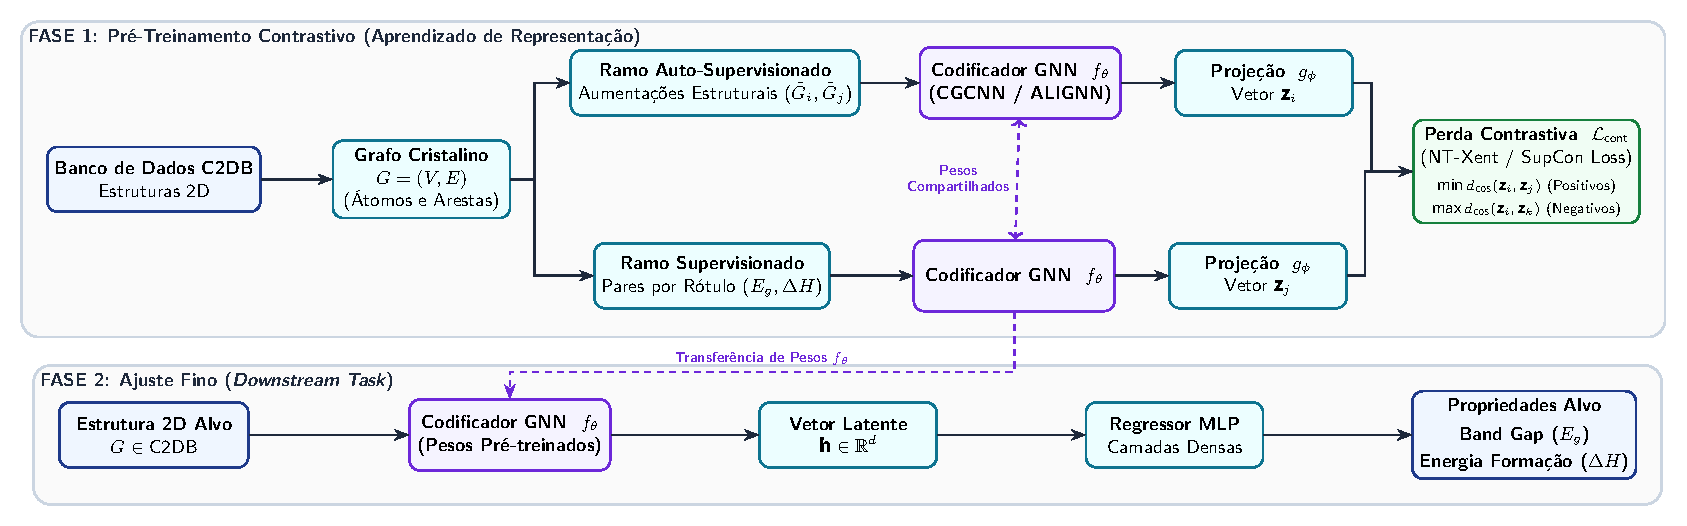
\includegraphics[width=\textwidth]{Figures/fluxograma.pdf}
\caption{Fluxograma da metodologia proposta para o desenvolvimento do modelo de aprendizado contrastivo aplicado a materiais bidimensionais. O pipeline inclui as etapas de pré-processamento de dados, treinamento contrastivo e avaliação das representações latentes obtidas.}
\end{figure}




Para pré-processamento, serão extraídas as estruturas cristalinas da base C2DB, convertendo-as em grafos atômicos com nós representando átomos e arestas representando ligações químicas. A etapa de aumentação envolverá a aplicação de transformações geométricas e topológicas que preservem as propriedades físicas dos materiais 2D, como pequenas perturbações atômicas e deformações elásticas no plano da monocamada. O treinamento contrastivo dependerá majoritariamnte da escolha da rede neural de grafos (como CGCNN ou Equiformer) e da função de perda contrastiva (como NT-Xent ou Contrastive Loss). A avaliação das representações latentes será realizada por meio de tarefas downstream, como a predição do \textit{bandgap} e da energia de formação, comparando o desempenho com modelos supervisionados tradicionais.



% ---
% Conclusão
% ---
% \chapter{Conclusão}
\chapter{Declaração sobre o Uso de Inteligência Artificial Generativa}

% Declaração sobre o uso de Inteligência Artificial Generativa. 
Durante a elaboração deste trabalho, o autor utilizou a ferramenta Copilot Student com a finalidade de revisão de linguagem aplicada a auto-completação de frases. Após esse uso, o autor revisou e editou  o conteúdo conforme necessário e assume integral responsabilidade pelo conteúdo do trabalho.

% ----------------------------------------------------------
% ELEMENTOS PÓS-TEXTUAIS
% ----------------------------------------------------------
\postextual


% ----------------------------------------------------------
% Referências bibliográficas
% ----------------------------------------------------------
\bibliographystyle{abntex2-alf}
\bibliography{references}

% ----------------------------------------------------------
% Glossário
% ----------------------------------------------------------
%
% Consulte o manual da classe abntex2 para orientações sobre o glossário.
%
%\glossary

% ----------------------------------------------------------
% Apêndices
% ----------------------------------------------------------

% ---
% Inicia os apêndices
% ---
% \begin{apendicesenv}

% Imprime uma página indicando o início dos apêndices
% \partapendices

% ----------------------------------------------------------
% \chapter{Título de Apêndice}
% ----------------------------------------------------------


% ----------------------------------------------------------
% \chapter{Título do Apêndice}
% ----------------------------------------------------------


% \end{apendicesenv}
% ---


% ----------------------------------------------------------
% Anexos
% ----------------------------------------------------------

% ---
% Inicia os anexos
% ---
% \begin{anexosenv}

% Imprime uma página indicando o início dos anexos
% \partanexos

% ---
% \chapter{Título do Anexo}
% ---

% \end{anexosenv}

\end{document}
